% Options for packages loaded elsewhere
\PassOptionsToPackage{unicode}{hyperref}
\PassOptionsToPackage{hyphens}{url}
%
\documentclass[
]{article}
\usepackage{amsmath,amssymb}
\usepackage{iftex}
\ifPDFTeX
  \usepackage[T1]{fontenc}
  \usepackage[utf8]{inputenc}
  \usepackage{textcomp} % provide euro and other symbols
\else % if luatex or xetex
  \usepackage{unicode-math} % this also loads fontspec
  \defaultfontfeatures{Scale=MatchLowercase}
  \defaultfontfeatures[\rmfamily]{Ligatures=TeX,Scale=1}
\fi
\usepackage{lmodern}
\ifPDFTeX\else
  % xetex/luatex font selection
\fi
% Use upquote if available, for straight quotes in verbatim environments
\IfFileExists{upquote.sty}{\usepackage{upquote}}{}
\IfFileExists{microtype.sty}{% use microtype if available
  \usepackage[]{microtype}
  \UseMicrotypeSet[protrusion]{basicmath} % disable protrusion for tt fonts
}{}
\makeatletter
\@ifundefined{KOMAClassName}{% if non-KOMA class
  \IfFileExists{parskip.sty}{%
    \usepackage{parskip}
  }{% else
    \setlength{\parindent}{0pt}
    \setlength{\parskip}{6pt plus 2pt minus 1pt}}
}{% if KOMA class
  \KOMAoptions{parskip=half}}
\makeatother
\usepackage{xcolor}
\usepackage[margin=1in]{geometry}
\usepackage{graphicx}
\makeatletter
\def\maxwidth{\ifdim\Gin@nat@width>\linewidth\linewidth\else\Gin@nat@width\fi}
\def\maxheight{\ifdim\Gin@nat@height>\textheight\textheight\else\Gin@nat@height\fi}
\makeatother
% Scale images if necessary, so that they will not overflow the page
% margins by default, and it is still possible to overwrite the defaults
% using explicit options in \includegraphics[width, height, ...]{}
\setkeys{Gin}{width=\maxwidth,height=\maxheight,keepaspectratio}
% Set default figure placement to htbp
\makeatletter
\def\fps@figure{htbp}
\makeatother
\setlength{\emergencystretch}{3em} % prevent overfull lines
\providecommand{\tightlist}{%
  \setlength{\itemsep}{0pt}\setlength{\parskip}{0pt}}
\setcounter{secnumdepth}{-\maxdimen} % remove section numbering
\usepackage[spanish]{babel}
\usepackage[fontsize=12pt]{scrextend}
\usepackage{geometry}
\geometry{letterpaper, margin=1in}
\usepackage{setspace}
\fontsize{13}{15}\selectfont
\usepackage{float}
\usepackage{colortbl}
\usepackage{booktabs}
\usepackage{longtable}
\usepackage{array}
\usepackage{multirow}
\usepackage{wrapfig}
\usepackage{float}
\usepackage{colortbl}
\usepackage{pdflscape}
\usepackage{tabu}
\usepackage{threeparttable}
\usepackage{threeparttablex}
\usepackage[normalem]{ulem}
\usepackage{makecell}
\usepackage{xcolor}
\ifLuaTeX
  \usepackage{selnolig}  % disable illegal ligatures
\fi
\IfFileExists{bookmark.sty}{\usepackage{bookmark}}{\usepackage{hyperref}}
\IfFileExists{xurl.sty}{\usepackage{xurl}}{} % add URL line breaks if available
\urlstyle{same}
\hypersetup{
  hidelinks,
  pdfcreator={LaTeX via pandoc}}

\author{}
\date{\vspace{-2.5em}}

\begin{document}

\begin{titlepage}
\centering



\vspace{2cm} % Espaciado vertical

{\Huge\bfseries Informe de Gastos\\ Primer Semestre 2023\par} 

\vspace{1.5cm}

{\Large HOSPITAL DR. GUSTAVO FRICKE \par} 

\vspace{2cm}

{\Large Fecha de elaboración: \today\par} % Fecha

\vfill % Llena el espacio vertical restante

{\large Autor: Fabián A. Rodríguez M.\par} % Autor

\end{titlepage}

\pagenumbering{arabic}

\newpage

\hypertarget{introducciuxf3n}{%
\subsection{INTRODUCCIÓN}\label{introducciuxf3n}}

El documento que se presenta a continuación fue elaborado como proyecto
final para el curso de capacitación ``Introducción a la ciencia de datos
con R''. Este curso fue impartido por el Instituto de Matemática, Física
y Estadística de la Facultad de Ingeniería y Negocios de la Universidad
de Las Américas.

En este informe, se analiza la información referente a las órdenes de
compra emitidas por el Hospital Gustavo Fricke durante el primer
semestre del 2023. La fuente primaria de los datos proviene de
Datos.gob, el repositorio de datos abiertos del Estado. Este repositorio
centraliza y ofrece datos públicos de manera clara y transparente, con
formatos abiertos, facilitando su búsqueda y utilización. Para aquellos
interesados en acceder directamente a la información utilizada, pueden
encontrarla en el siguiente
\href{https://chc-oc-files.s3.amazonaws.com/entcode/2023/Sem1/6936.7z}{enlace}.

Es importante destacar que la información específica sobre las órdenes
de compra es suministrada por la plataforma transaccional de
ChileCompra, www.mercadopublico.cl. Esta plataforma congrega tanto la
demanda de los entes públicos como la oferta de los proveedores en un
solo espacio.

En cuanto al Hospital Dr.~Gustavo Fricke, es pertinente mencionar que es
uno de los hospitales autogestionados de alta complejidad del país.
Representa el establecimiento de mayor envergadura dentro de la Red del
Servicio de Salud Viña del Mar Quillota. En 2014, el hospital celebró su
60° aniversario y logró la distinción de Hospital Acreditado en Calidad.
Estos logros reflejan el esfuerzo y compromiso continuo de sus
funcionarios para brindar una atención sanitaria de calidad a la
población.

\newpage

\hypertarget{gasto-por-tamauxf1o-de-proveedor-en-el-primer-semestre-del-auxf1o-2023}{%
\subsubsection{GASTO POR TAMAÑO DE PROVEEDOR EN EL PRIMER SEMESTRE DEL
AÑO
2023}\label{gasto-por-tamauxf1o-de-proveedor-en-el-primer-semestre-del-auxf1o-2023}}

Para el presente informe, hemos establecido como objetivo principal
extraer información referente a los tipos de proveedores con los cuales
se realizan transacciones, basándonos en la clasificación de tamaño del
proveedor (TamanoProveedor). Para determinar el valor de las órdenes de
compra, hemos optado por seleccionar el valor total de cada ítem
(MontoTotalItem). Es importante mencionar que, con el fin de facilitar
la comprensión de los datos, hemos representado los valores monetarios
en millones.

\begin{table}[H]

\caption[ssss]{\label{tab:tabla-TamanoProveedor}Gastos por Tamaño de Proveedor}
\centering
\begin{tabular}[t]{>{}l>{}r}
\toprule
\textcolor[HTML]{4A90E2}{\textbf{Tamaño de Proveedor}} & \textcolor[HTML]{4A90E2}{\textbf{Monto Neto}}\\
\midrule
\textbf{\cellcolor[HTML]{B3E2CD}{\textcolor{gray}{\textbf{Grande}}}} & \textbf{\cellcolor[HTML]{B3E2CD}{\textcolor{gray}{\textbf{8,389}}}}\\
\textbf{\cellcolor[HTML]{FDCDAC}{\textcolor{gray}{\textbf{Mediana}}}} & \textbf{\cellcolor[HTML]{FDCDAC}{\textcolor{gray}{\textbf{605}}}}\\
\textbf{\cellcolor[HTML]{CBD5E8}{\textcolor{gray}{\textbf{Micro}}}} & \textbf{\cellcolor[HTML]{CBD5E8}{\textcolor{gray}{\textbf{195}}}}\\
\textbf{\cellcolor[HTML]{F4CAE4}{\textcolor{gray}{\textbf{NoClasificado}}}} & \textbf{\cellcolor[HTML]{F4CAE4}{\textcolor{gray}{\textbf{787}}}}\\
\textbf{\cellcolor[HTML]{E6F5C9}{\textcolor{gray}{\textbf{Pequeña}}}} & \textbf{\cellcolor[HTML]{E6F5C9}{\textcolor{gray}{\textbf{616}}}}\\
\bottomrule
\end{tabular}
\end{table}
\newpage

\hypertarget{gasto-acumulado-por-tamauxf1o-de-proveedor-en-el-primer-semestre-del-auxf1o-2023}{%
\subsubsection{GASTO ACUMULADO POR TAMAÑO DE PROVEEDOR EN EL PRIMER
SEMESTRE DEL AÑO
2023}\label{gasto-acumulado-por-tamauxf1o-de-proveedor-en-el-primer-semestre-del-auxf1o-2023}}

Para complementar la comprensión sobre las transacciones realizadas
durante el primer semestre del 2023 con diferentes tipos de proveedores,
se ha elaborado un gráfico de área que muestra la evolución acumulada
mes a mes del valor total de las órdenes de compra, segmentado según el
tamaño del proveedor. Dicho gráfico permite visualizar la dinámica y
tendencia en las transacciones, ayudando a identificar patrones o
cambios significativos en los montos de compra a lo largo de este
período. Al igual que en la tabla anterior, los valores en el gráfico
están representados en millones para una interpretación más directa y
clara de las cifras.

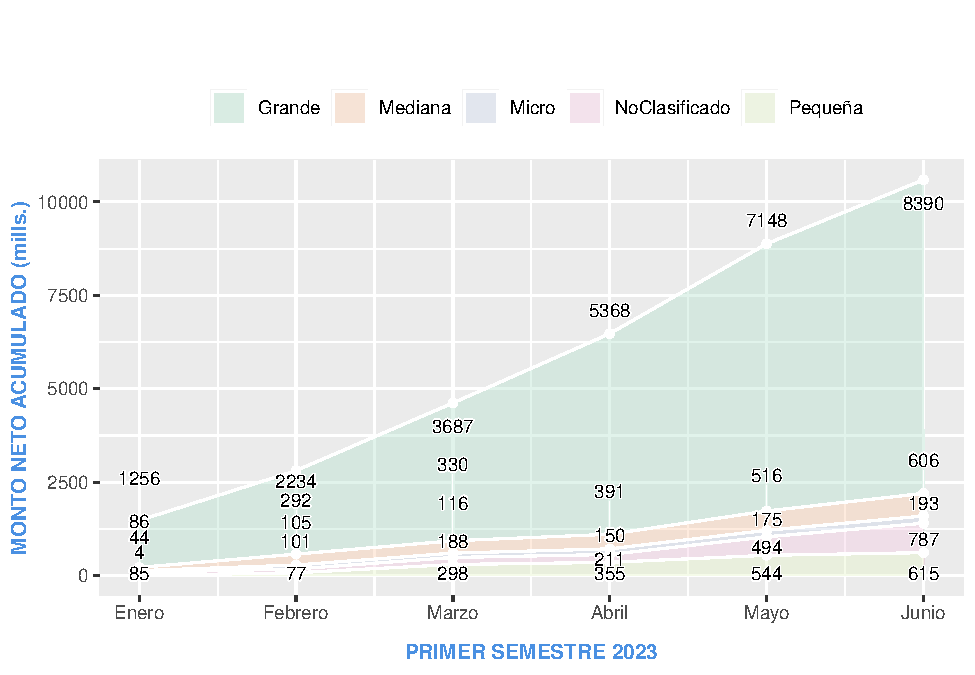
\includegraphics{GastoPrimerSemestre2023_files/figure-latex/grafico-acumulado-1.pdf}
\newpage

\hypertarget{gasto-mensual-en-el-primer-semestre-del-auxf1o-2023}{%
\subsubsection{GASTO MENSUAL EN EL PRIMER SEMESTRE DEL AÑO
2023}\label{gasto-mensual-en-el-primer-semestre-del-auxf1o-2023}}

A continuación, se presenta un análisis complementario que busca
sintetizar aún más la información, despojando la diferenciación por
tamaño de proveedor. En el gráfico de área subsiguiente, se visualiza la
evolución del gasto mensual total durante el primer semestre del 2023.
Esta perspectiva nos brinda una vista macro de los gastos del Hospital,
ofreciendo una apreciación directa de la dinámica de compras en el
transcurso de los meses, sin entrar en la segmentación por tipo de
proveedor. De esta forma, se busca entender el comportamiento global de
los gastos y determinar momentos de mayor o menor actividad de compra.

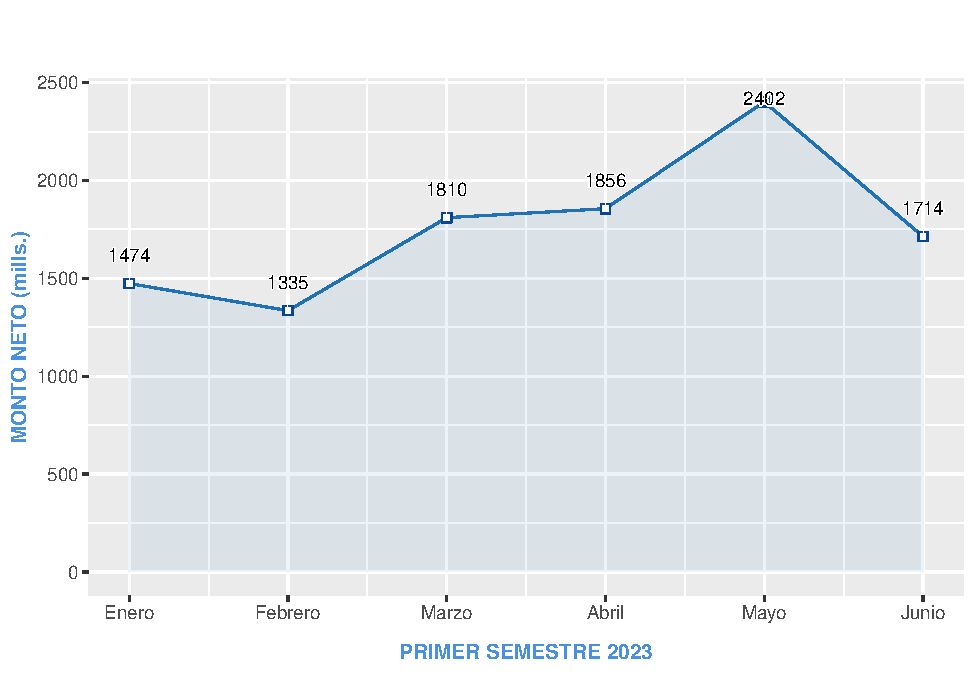
\includegraphics{GastoPrimerSemestre2023_files/figure-latex/grafico-mes-1.pdf}
\newpage 

\hypertarget{conclusiuxf3n}{%
\subsubsection{CONCLUSIÓN}\label{conclusiuxf3n}}

Después de analizar los datos presentados en los gráficos, se puede
apreciar ciertos patrones y tendencias en los gastos del Hospital
durante el primer semestre del 2023.

En lo que respecta a la distribución del gasto por tamaño de proveedor,
los proveedores grandes lideran claramente con un monto de 8,389
millones, seguidos a cierta distancia por aquellos que no están
clasificados (787 millones), las empresas medianas (605 millones) y las
pequeñas (616 millones). Las microempresas, como era de esperarse,
presentan el menor gasto, sumando a la cuenta 195 millones. Este
desglose evidencia una concentración significativa de gastos con
proveedores de gran tamaño, lo que puede ser indicativo de contratos o
transacciones más grandes y frecuentes con este tipo de proveedores.

Por otro lado, al examinar la evolución mensual del gasto durante el
primer semestre, se observa un aumento progresivo desde enero (1,474
millones) a mayo (2,402 millones), con una pequeña disminución en junio
(1,714 millones). Febrero y marzo muestran gastos similares de 1,335 y
1,810 millones, respectivamente, y abril refleja un gasto de 1,856
millones. El mes de mayo destaca como el de mayor gasto, siendo este un
punto de interés que podría requerir un análisis más detallado para
entender las razones detrás de este pico.

En resumen, el Hospital ha mantenido una tendencia creciente en sus
gastos durante la primera mitad del 2023, con una notable preferencia
por los proveedores de gran tamaño. Esta información es esencial para la
toma de decisiones y la planificación financiera futura, además de
establecer estrategias de negociación y contratación con diferentes
tipos de proveedores.

\end{document}
